\section{Produkt}
Nedan följer de resultaten teamet har tagit fram i form av den utvecklade produkten. Detta resultat relaterar till frågeställning 1\ref{fs:fs_1}. Produkten som utvecklats kan delas upp i tre olika delar, som kan ses tidigare i figur \ref{fig:konceptarkitektur}. Dessa delar är kontroller, UI och service, där den sistnämnda implementerades som en del av Cybercoms backend.


\subsection{Service}
När kraven för produkten samlades in tidigt i projektet var det tydligt att kunden ville ha ett system för att ansluta sig till fler är ett spel. Detta betyder att flera instanser av UI:t ska kunna vara igång samtidigt och att användaren ska ha möjlighet att välja vilket spel denne vill ansluta sig till. Detta implementerades med hjälp av en \textit{Service} i Cybercoms backend. Denna service registrerar när nya instanser skapas eller tas bort i UI:t och skickar denna information vidare till kontrollern. Kontrollern kan sedan visa dessa instanser, vilket kan ses i figur \ref{fig:controller_instances}.

\subsection{Kontroller}
Kontrollern i produkten som utvecklats är gränsnittet som används för att styra en spelare på spelplanen i UI:t. Som det nämns ovan kan användaren i en lista se och välja vilken spelinstans som ska anslutas till\ref{fig:controller_instances}. När användaren valt sin instans finns möjligheten att anpassa namnet och utseendet av sin spelare, som kan ses i figur \ref{fig:controller_selection}. När användaren är nöjd med utseendet av sin spelare kan denne ansluta till spelsessionen genom \textit{Join}-knappen. Efter detta är kontrollern ansluten till den spelinstans som valdes innan. Användaren kan styra sin spelare på planen genom att luta mobiltelefonen, och använda eventuella funktioner i spelet genom att klicka på deras tillhörande knapp. Exempel på detta kan ses i \ref{fig:controller_gamescreen}. Det spelläge som visas i denna figur, \textit{Knockoff}, har endast en extra funktion, \textit{Super Heavy}, som användaren kan använda sig av. Användaren kan också se sitt egna namn, svarstid och utseende, kalibrera sin rörelsesensor och lämna spelet från denna skärm. 


\begin{figure}[h]
    \centering
    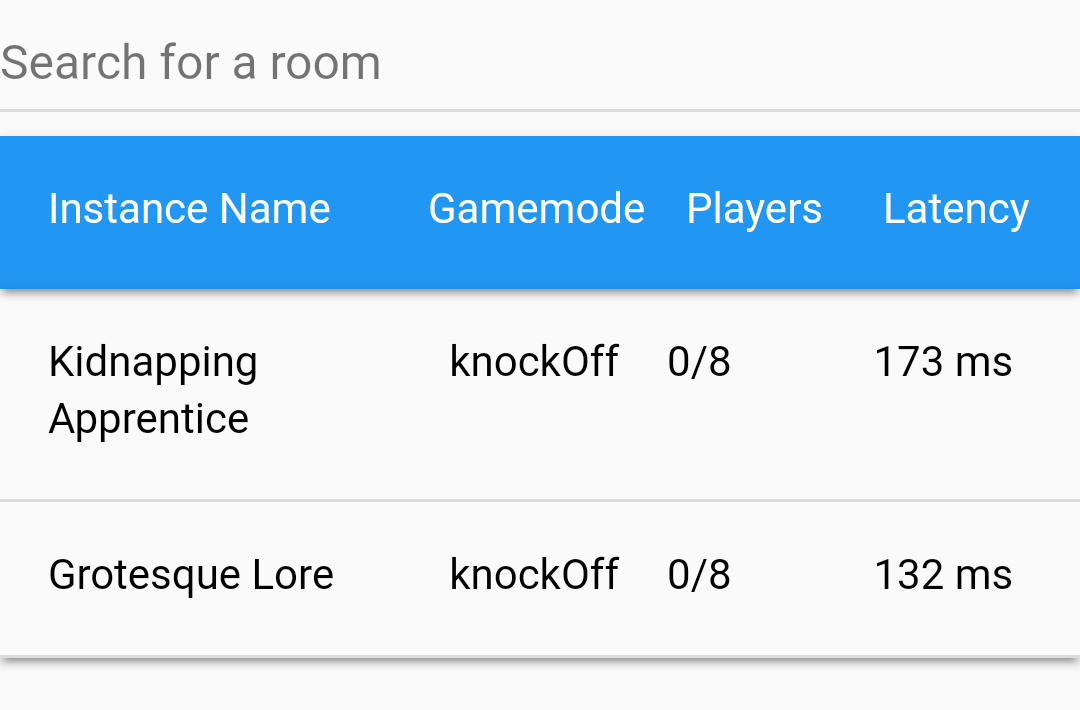
\includegraphics[scale=0.3]{controller_instances}
    \caption{Exempel hur visningen av instanser ser ut på kontrollern}
    \label{fig:controller_instances}
\end{figure}

\begin{figure}[h]
    \centering
    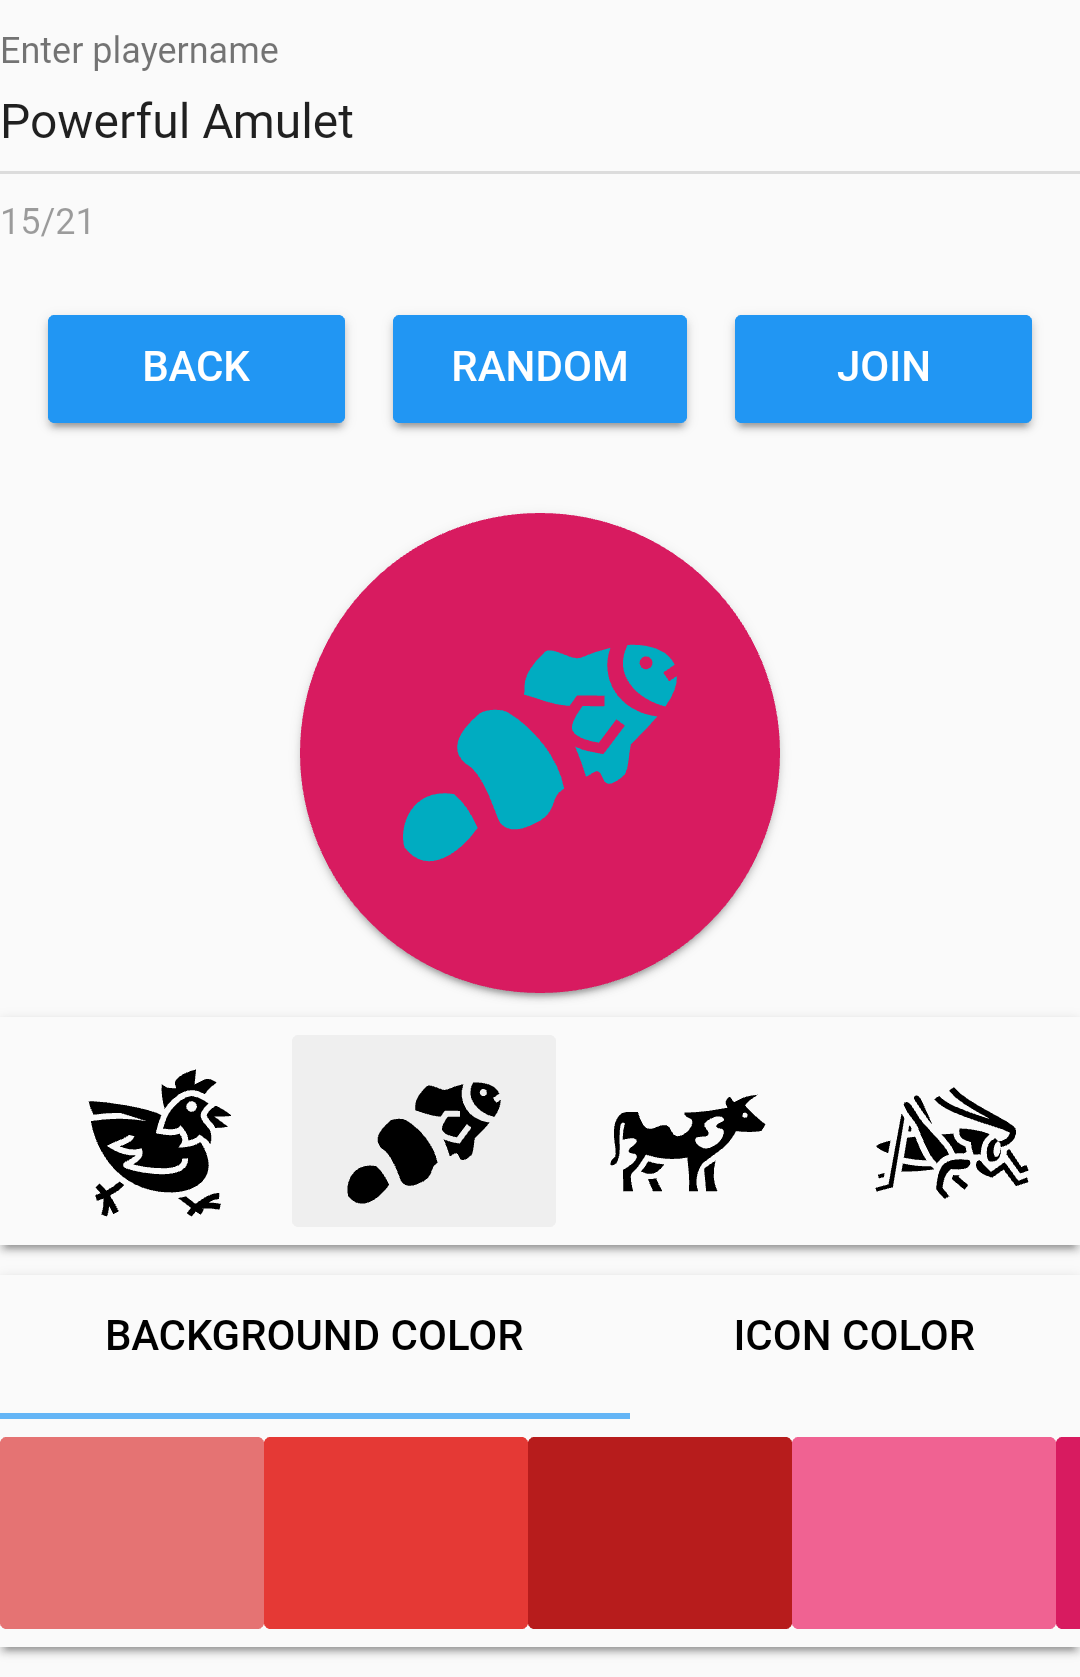
\includegraphics[scale=0.2]{controller_selection}
    \caption{Skärm för att anpassa sin spelare innan anslutning till en spelinstans}
    \label{fig:controller_selection}
\end{figure}

\begin{figure}[h]
    \centering
    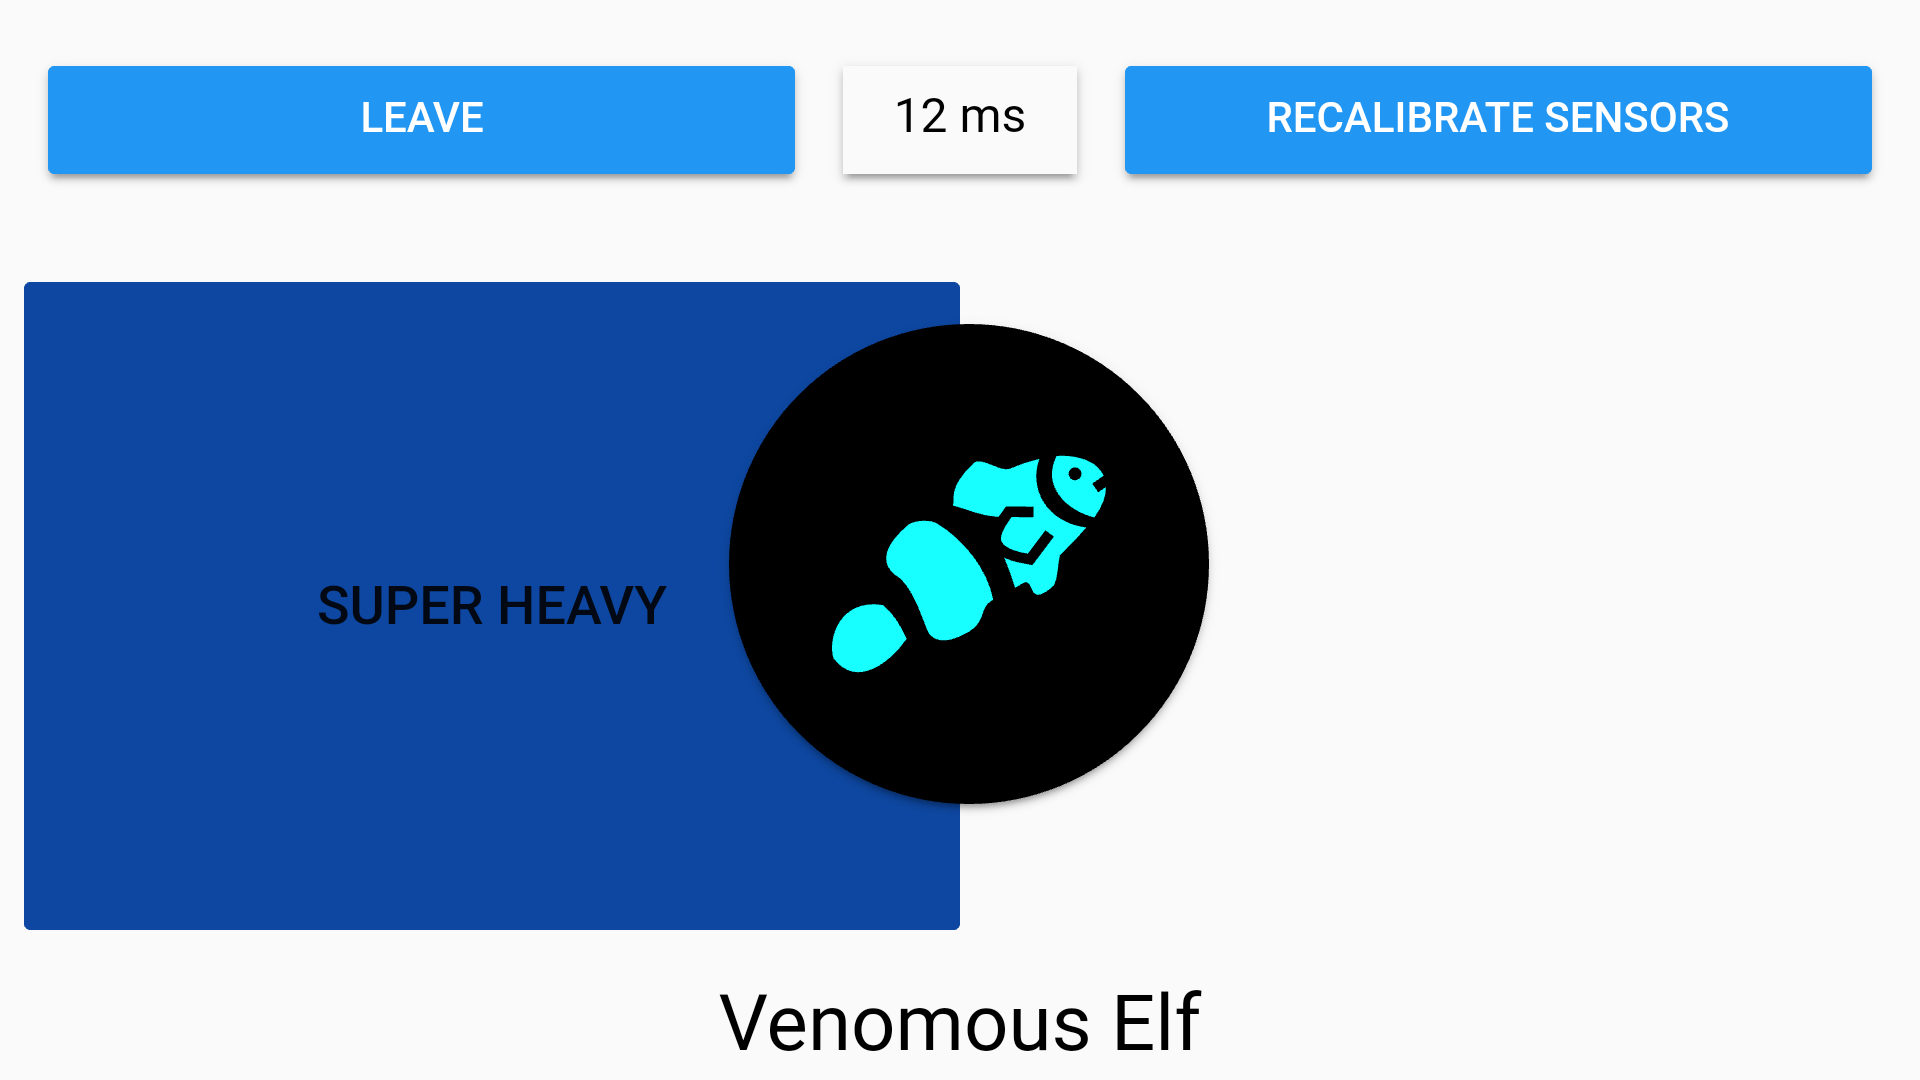
\includegraphics[scale=0.15]{controller_gamescreen}
    \caption{Skärmdump av kontrollern i spelläget \textit{Knockoff}}
    \label{fig:controller_gamescreen}
\end{figure}

\subsection{UI och nätverk}
Denna del av produkten ansvarar för att välja vilket spelläge som ska spelas, samt köra och visa spelet för alla användare. Spellägena som finns är fokuserade på en spelplan man ser överifrån där varje spelare styr en egen cirkel. Nedan i figur \ref{fig:ui-dodgebot} och figur \ref{fig:ui-knockoff} kan man se två av de spellägen som finns att välja på. Båda spellägena går ut på att styra sin cirkel för att överleva spellägets hinder. För att användarna ska ha god möjlighet till att undika dessa hinder behöver spelet svara responsivt till input från kontrollern. Detta var en utmaning för gruppen då datan som skickas från kontrollern till spelet skickas över nätverk och därför påverkas av nätverkets svarstid. Eftersom spelet spelas i realtid är det alltså viktigt att användarens input också påverkar spelet i realtid. För att spelupplevelsen ska vara responsiv har därför gruppen jobbat mycket med att optimera hur mycket data som skickas via nätverket. Detta uppnås genom att kontrollern enbart skickar data då sensorvärdena uppdaterats. Sensorvärdena är också avrundade till närmaste heltal då gruppen ansåg att ytterligare upplösning inte skulle leda till en bättre spelupplevelse. Utöver åtgärderna på kontrollern kalibrerade också gruppen hantering av sensordata på UI:t. Kalibreringen skedde manuellt tills gruppen var nöjd med känslan att styra en spelare. I verkligheten betydde detta en styrning som direkt reagerar på ny input, men också tar hänsyn till tidigare värden som tagit emot. Detta ledde till robust styrsystem som ger mjuka rörelser i spelet och klarar av eventuella nätverksstörningar utan att spelaren tappar kontrollen. 


\begin{figure}[t]
    \centering
    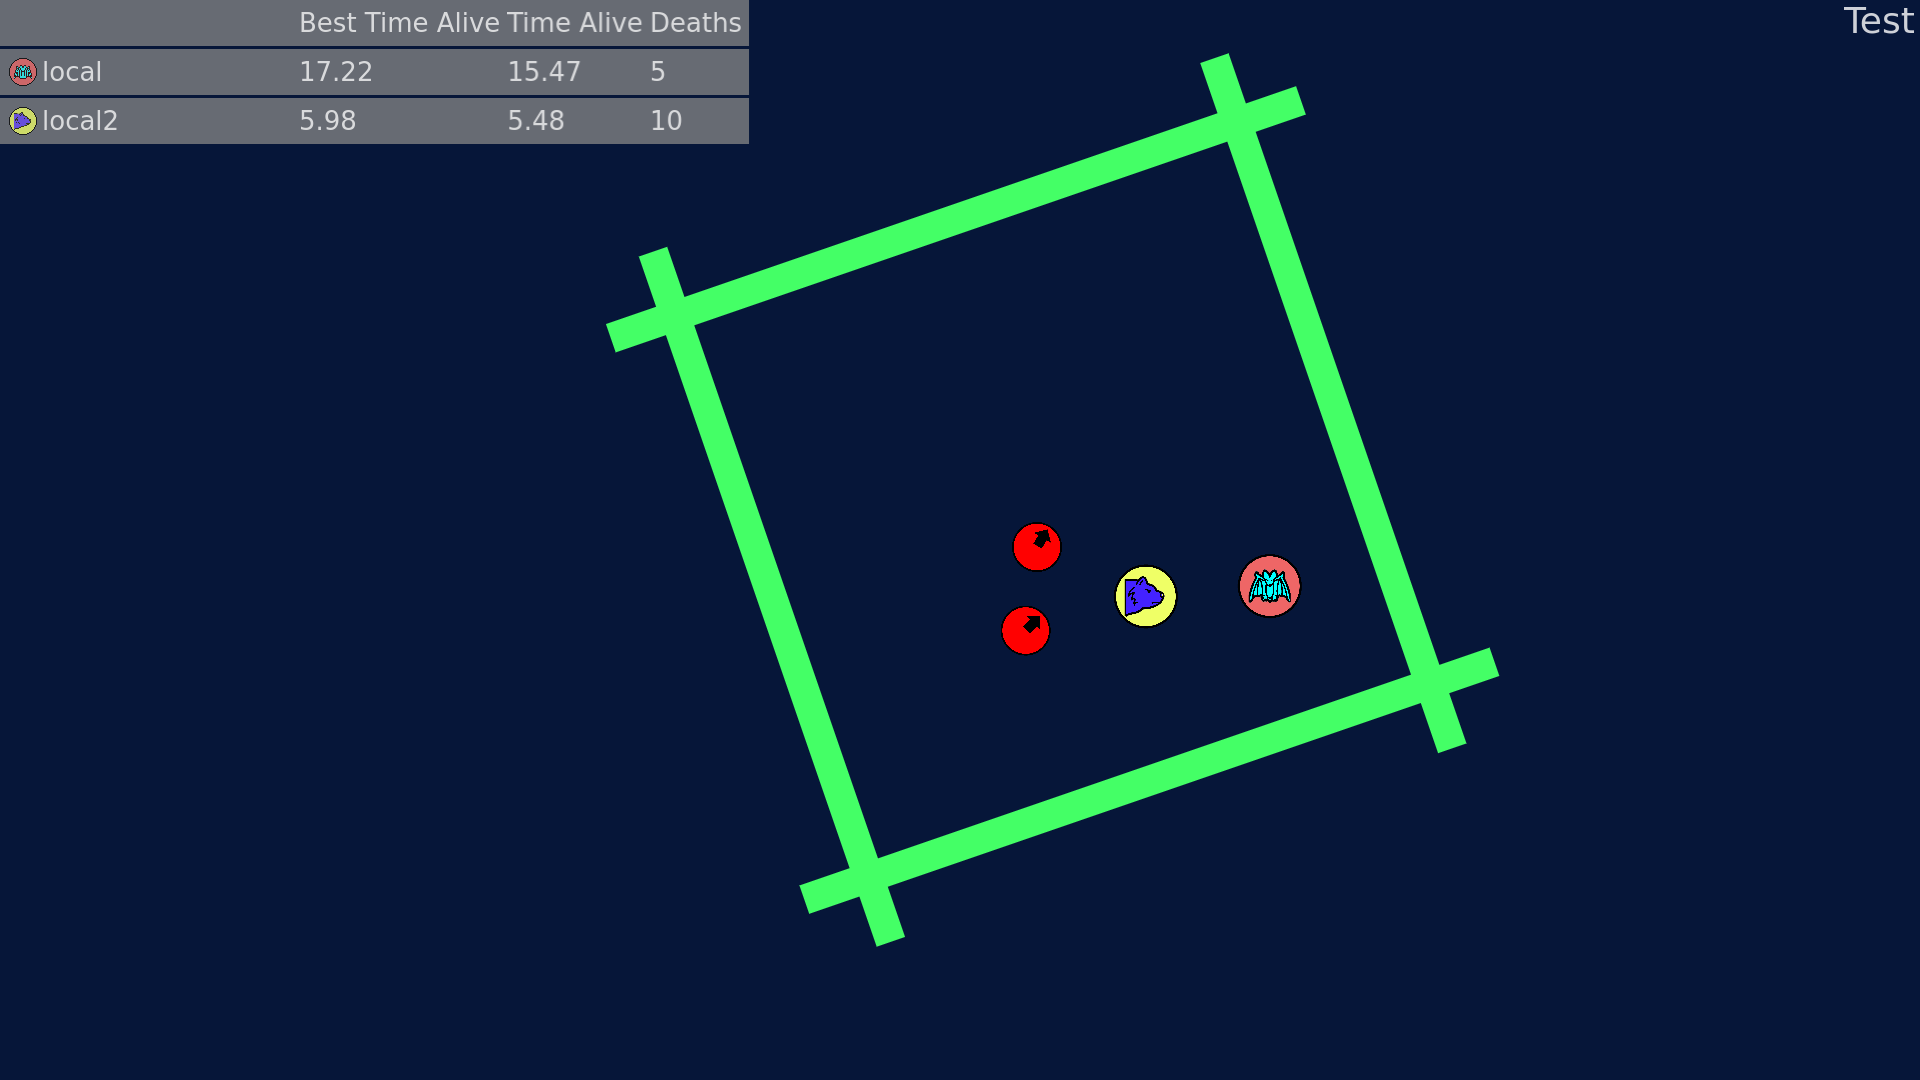
\includegraphics[scale=0.2]{ui-dodgebot}
    \caption{Skärmdump av UI:t i spelläget \textit{Dodgebot}}
    \label{fig:ui-dodgebot}
\end{figure}

\begin{figure}[b]
    \centering
    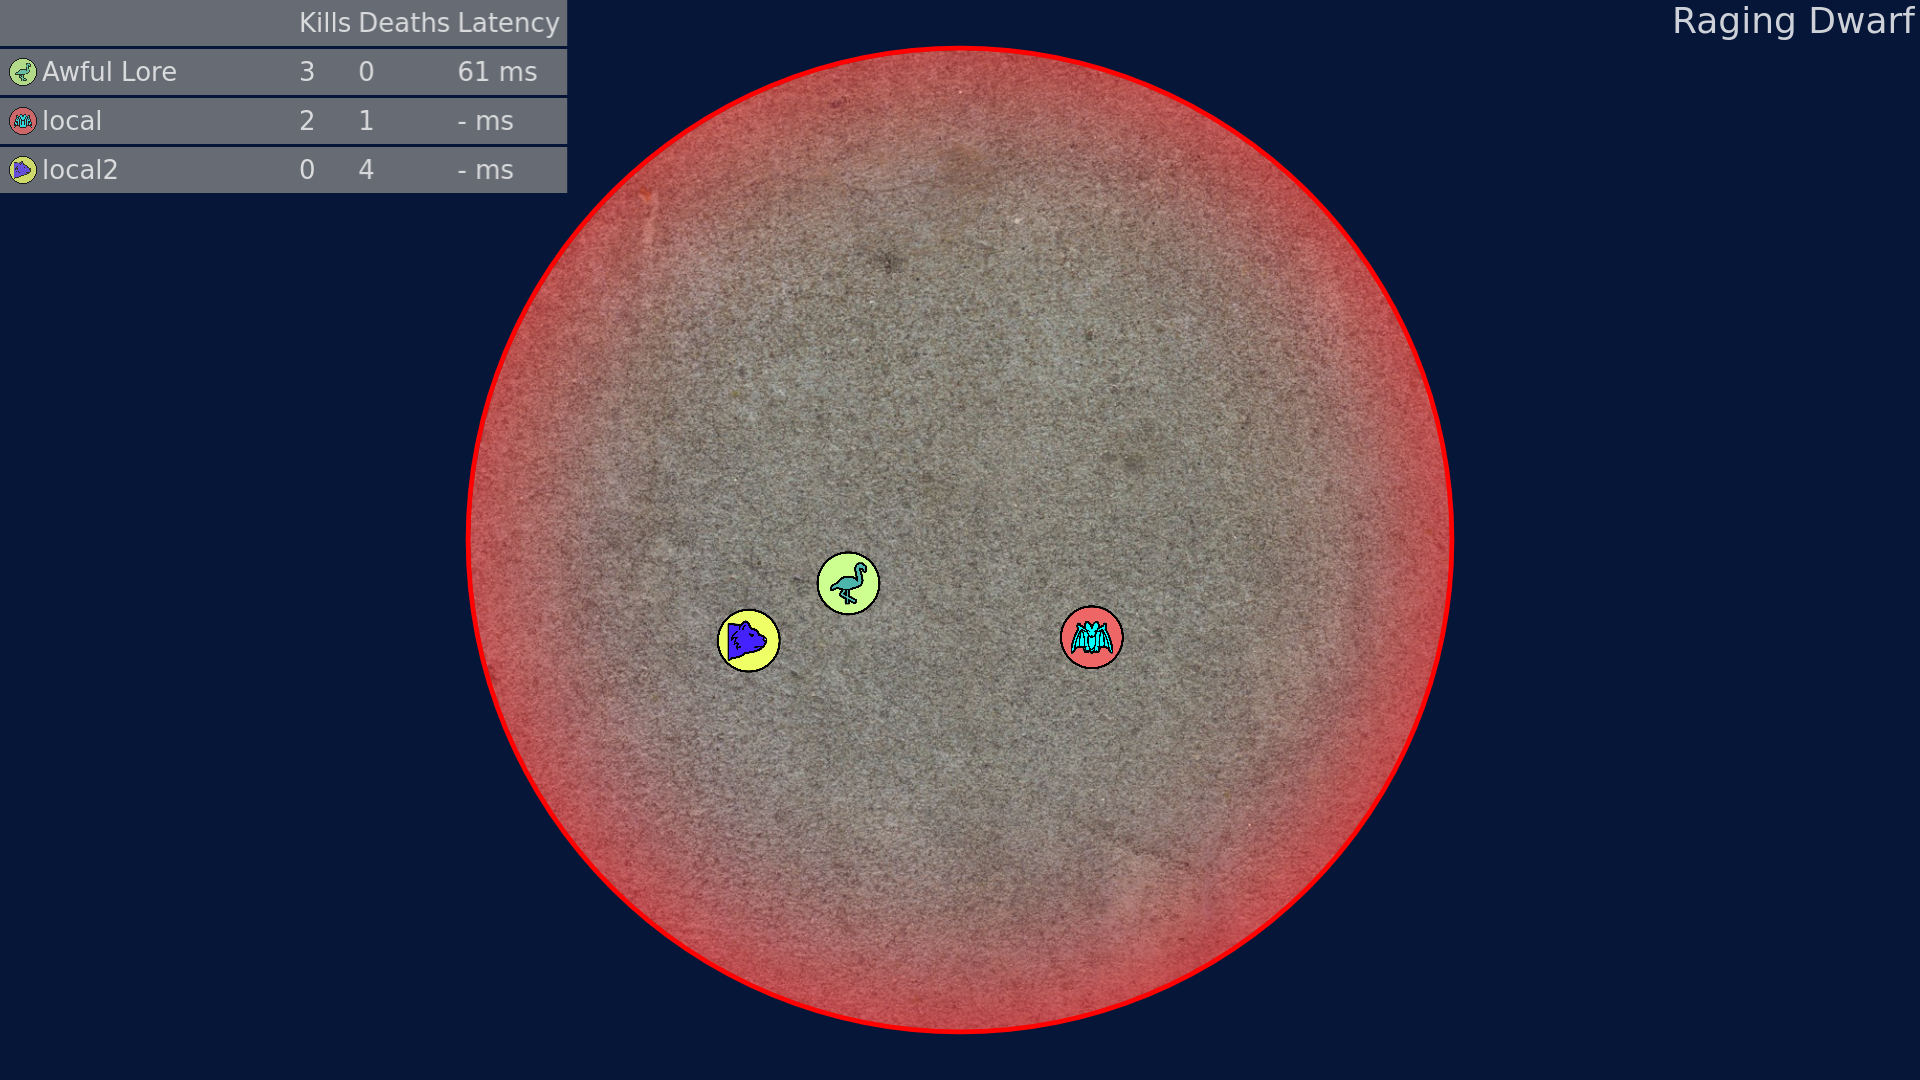
\includegraphics[scale=0.2]{ui-knockoff}
    \caption{Skärmdump av UI:t i spelläget \textit{Knockoff}}
    \label{fig:ui-knockoff}
\end{figure}